\documentclass[10pt,twocolumn,letterpaper]{article}

\usepackage{cvpr}
\usepackage{times}
\usepackage{epsfig}
\usepackage{graphicx}
\usepackage{amsmath}
\usepackage{amssymb}

% Include other packages here, before hyperref.

% If you comment hyperref and then uncomment it, you should delete
% egpaper.aux before re-running latex.  (Or just hit 'q' on the first latex
% run, let it finish, and you should be clear).
\usepackage[pagebackref=true,breaklinks=true,letterpaper=true,colorlinks,bookmarks=false]{hyperref}

\cvprfinalcopy % *** Uncomment this line for the final submission

\def\cvprPaperID{****} % *** Enter the CVPR Paper ID here
\def\httilde{\mbox{\tt\raisebox{-.5ex}{\symbol{126}}}}

% Pages are numbered in submission mode, and unnumbered in camera-ready
\ifcvprfinal\pagestyle{empty}\fi
\begin{document}

%%%%%%%%% TITLE
\title{Convolutional Neural Network to Detect Equivalent Questions in Online Forums  \\ DL-IC 2018 Project} 

\author{Luca Scannapieco\\
Politecnico di Milano\\
{\tt\small luca.scannapieco@mail.polimi.it}
% For a paper whose authors are all at the same institution,
% omit the following lines up until the closing ``}''.
% Additional authors and addresses can be added with ``\and'',
% just like the second author.
% To save space, use either the email address or home page, not both
\and
Nicola Sosio\\
Politecnico di Milano\\
{\tt\small nicola.sosio@mail.polimi.it}
\and
Maria Chiara Zaccardi\\
Politecnico di Milano\\
{\tt\small mariachiara.zaccardi@mail.polimi.it}
}

\maketitle
%\thispagestyle{empty}

%%%%%%%%% ABSTRACT
\begin{abstract}
   In the context of online forums, although two questions may seem very different in terms of vocabulary, length and syntax, they may eventually ask the same thing. In this work, we try to detect semantically equivalent questions using a simple Convolutional Neural Network (CNN). The proposed CNN generates distributed vector representations for pairs of questions and score them using a similarity metric. This work is the replication of \cite{bogdanova2015detecting}: we basically try to perform the same experiments and compare our results with theirs. The replication turned to be not straightforward since some crucial implementation details are missing in the Bogdanova et al.'s description. Hence, we have found quite stimulating to replicate this paper filling the holes with our own ideas. In particular, our efforts focused mainly on the following three aspects that were not explicitly treated in the paper: unequal text length, the type of convolution and the training of in-domain word embeddings. The final results we obtained are quite close to the our target; whereas the optimal parameters values of the network are quite different from \cite{bogdanova2015detecting}.
\end{abstract}

%%%%%%%%% BODY TEXT
%------------------------------------------------------------------------
\section{Introduction}
Natural Language Processing (NLP) is just one of several fields emerging from Artificial Intelligence. In NLP we want the machine to process and analyze large amount of natural language data to accomplish very interesting tasks (such as Sentiment Analysis, Language Identification and many others). Nowadays, these tasks are plenty and many works on them has been already carried out \footnote{Here is a very interesting repository collecting several NLP tasks along with their main references: \\ \url{https://github.com/Kyubyong/nlp_tasks}}. In this paper, we focus on the task of predicting whether two questions from an online forum are semantically equivalent, i.e. they can be answered by the exact same answer. This can be a very useful tool for Question-Answering community sites as they typically want to keep their databases as less redundant as possible, so to make the searches of their users both faster and more effective. Furthermore, they want to keep people from wasting their time in answering already solved questions. \\
The main contribution of this work is \cite{bogdanova2015detecting}. In their work, Bogdanova et al. propose a simple Convolutional Neural Network (CNN) to detect semantically equivalent questions. The proposed network first transforms words into \emph{word embeddings} and then applies a convolutional layer which generates question-wide vectors representations. Finally, pairs of questions are scored using a similarity function. The most interesting experimental result is the evaluation of in-domain word embeddings versus the word embeddings generated using all of the English Wikipedia. In particular, they shown that domain-specific word embeddings achieve higher performances. \\
In general, the results obtained by our implementation are very close to the ones of the replicated paper. Surprisingly, as we will discuss in Section 4, the main differences in the results are about the optimal hyper-parameter values of the network.\\
The authors of the paper accurately described the architecture of the network, but many crucial details of the model are missing in their description. Hence, we have found quite stimulating to replicate this paper filling the holes with our own ideas. In particular, our efforts focused mainly on the following three aspects that were not explicitly treated in the paper: 
    \paragraph{Handling questions of different sizes.}
    Bogdanova et al. explicitly state that the different sizes of questions is one of the main challenges of their work. Nevertheless, they do not specify the way they solved this issue. We, therefore, tried to fix the length of each question to the \textbf{maximum} and to the \textbf{mean} length of all the questions. The first approach resulted to yield the greater accuracy.
    \paragraph{The type of convolution.}
    For the implementation of our network we used a 1-dimensional convolution. Indeed, text can be seen as images with the input maps having only one dimension (height, without width) corresponding to the question length and where the number of input maps is nothing but the size of the word embeddings. The type of convolution represents another missing detail of \cite{bogdanova2015detecting}.    
    \paragraph{The training of in-domain word embeddings.}
    The paper does not provide any information about the model used to train in-domain word embeddings. Initially, we tried to build our own \emph{word2vec} model \cite{mikolov2013distributed} to generate word-embeddings using as training data the same dataset used to train the main network \footnote{To do so we followed this good tutorial: \url{http://adventuresinmachinelearning.com/word2vec-keras-tutorial/}}. However, the training of this network turned out to be very slow and resulting embeddings perfomed poorly. \\
    We, then, decided to use Gensim, a very simple library which generates word-embeddings given the training data. The resulting embeddings performed very well, allowing the main network to achieve up to 90\% of accuracy on the validation set.

%------------------------------------------------------------------------
\section{Related work}
Detecting text similarities is a problem which was probably born before deep learning. In \cite{gomaa2013survey}, Gomaa et al. survey existing algorithms for both lexical and semantical text similarity. All these algorithms have nothing to do with Neural Networks, and can therefore be used as baselines to understand how much deep learning has improved the state-of-the-art.\\
In \cite{kim2014convolutional}, Kim proposes a very simple CNN architecture trained on top of pre-trained word vectors. He experimented the same network on 7 different sentence-level classification tasks and, for each task, he compared the obtained results with the state-of-the-art: the CNN approach improved upon the state-of-the-art on 4 out of 7 tasks. Moreover, he proposes a slight modification of the network with 2 channels of word vectors: one that is kept static during the training and one that is fine-tuned via backpropagation. Although not explicitly stated, we think this has been the main contribution of \cite{bogdanova2015detecting} as the network architecture is pretty much the same. The Kim's architecture represents the state-of-the-art on many NLP sentence classification tasks and it is often used as a layer of more complex networks which need to compute sentence-level distributed vectors representation. For example, in \cite{severyn2015learning}, the network is used as a fundamental preprocessing step in a learning-to-rank algorithm. \\
A different but still interesting approach to the problem of text classification, is described in \cite{zhang2015character}. In this article, the authors explore treating text as a kind of raw signal at character level, and applying temporal (one-dimensional) Convolutional Network to it.\\
Different CNN architectures are used for solving a wide range of NLP tasks and many encouraging results have been already achieved. Yih et al. \cite{yih2014semantic} introduced a novel semantic similarity model based on a CNN architecture for the task of answering single-relation factual questions. Hu et al. \cite{hu2014convolutional} proposed a CNN architecture for hierarchical sentence modeling and sentence matching. Convolution has been also used by Dos Santos et al. \cite{dos2014deep} for sentiment analysis of short texts that jointly uses character-level, word-level and sentence-level information.\\
To tackle the problem of sentences with different lengths, Socher et al. \cite{socher2011dynamic}, introduce a novel dynamic pooling layer which computes a fixed-sized representation from the variable-sized matrices. Another approach could be to use Long Short-Term Memory (LSTM), generating fixed-sized states from the input sentences (as done in \cite{tai2015improved}).\\
In \cite{zhou2015c}, a novel model called C-LSTM is presented: this model stack CNN and LSTM in a unified architecture for semantic sentence modeling. In this way, they are able to combine the strengths of both architectures. In particular, they apply CNN to text data and feed consecutive window features directly to LSTM. In this way, their architecture enables LSTM to learn long-range dependencies from higher-order sequential features.
%------------------------------------------------------------------------
\section{Proposed approach}
In this section we present our strategy for detecting semantically equivalent questions. In subsection 3.1, we describe in detail the architecture of the Neural Network. Then, in subsequent subsections, we focus on the decisions we have made about the things left unspecified by Bogdanova et al.
%-------------------------------------------------------------------------
\subsection{Neural Network Architecture}
As detailed in Figure \ref{fig:network}, the input for the network is tokenized text strings of the two questions. In the first step, the CNN transforms words into real valued feature vectors, also known as \emph{word embeddings}. Next, a convolutional layer is used to construct two distributed vector representations $\vec{r}_{q1}$ and $\vec{r}_{q2}$, one for each input question. Finally, the CNN computes a similarity score between $\vec{r}_{q1}$ and $\vec{r}_{q2}$. Pairs of questions with similarity above a threshold are considered duplicates. Each of these step is explained in more details in the following.
\begin{figure}[t]
\begin{center}
%\fbox{\rule{0pt}{2in} \rule{0.9\linewidth}{0pt}}
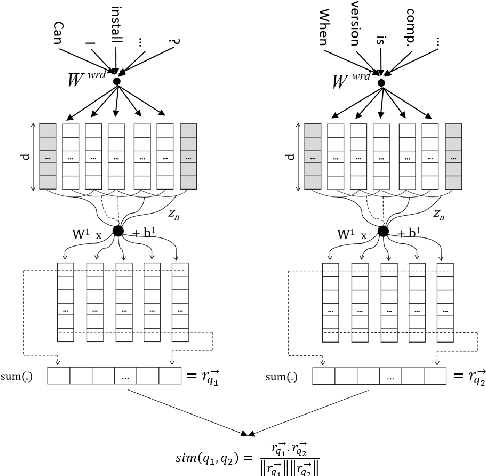
\includegraphics[width=0.8\linewidth]{img/network.png}
\end{center}
\caption{The network architecture.}
\label{fig:network}
%\label{fig:onecol}
\end{figure}

\subsubsection{From text to embeddings}
The first layer of the network transforms words into representations that capture syntactic and semantic information about the words. The initialization of this layer requires two strictly correlated objects:
\begin{itemize}
\item \textbf{The vocabulary}: a dictionary $V$ associating each word of the corpora used to train the embeddings to an integer index. In this vocabulary, we must also reserve an index for all the words which are not present in the vocabulary. Best practices suggest to have the index $0$ for the \emph{unknown} words and then having the other indexes ordered by most common words.
\item \textbf{The pre-trained word-embeddings}: a matrix $W_0 \in \mathbb{R}^{|V| \times d}$ where $d$ is the size the word embeddings. In this matrix, the $i$-th row corresponds to the word embedding of the $i$-th word in the vocabulary.
\end{itemize}•
The input of this layer is a 1-dimensional vector $\vec{q}=[w_1, w_2, ... , w_N]$ where the element $w_i$ is an integer number corresponding to the index of the $i$-th word of the question. We initialize the layer with our pre-trained word embeddings \footnote{either the word embeddings trained by us or the those trained by Google}, which is the matrix $W_0$. This layer, for each index $w_i$ of the input vector, retrieves the corresponding vector representation $\vec{r}^{w_i}$ in matrix $W_0$. Hence, the output is a matrix $X_0 \in \mathbb{R}^{N \times d}$.\\
Notice that if we use pre-trained word embeddings, the values of both the $d$ and $|V|$ have been already decided. These two hyper-parameters should have been tuned by people who trained the matrix $W_0$. Therefore, we will discuss them later when we will describe the training of in-domain word embeddings.  Even the question length $N$ is something that will be treated later on.

\subsubsection{The convolution}
We use a convolutional layer to compute the question-wide distributed vector representations $\vec{r}_{q1}$ and $\vec{r}_{q2}$. For each question, the convolutional layer first produces local features around each word in the question. Then, it combines these local features using a sum operation to create a fixed-sized feature vector (representation) for the question.\\
Given a question $q$, the convolutional layer applies a matrix-vector operation to each window of size $k$ of successive windows in $\vec{q}_{emb} = [\vec{r}^{w_1},\vec{r}^{w_2}, ..., \vec{r}^{w_N}]$. Let us define the vector $\vec{z}_n \in \mathbb{R}^{dk}$ as the concatenation of a sequence of $k$ word embeddings, centralized in the $n$-th word:
\begin{center}
$\vec{z}_n = [\vec{r}^{w_{n-(k-1)/2}},..., \vec{r}^{w_n}, ...,\vec{r}^{w_{n+(k-1)/2)}}]^T$
\end{center}•
The convolutional layer computes the $j$-th element of the vector $\vec{r}_{q1} \in \mathbb{R}^{cl_u}$ as follows: 
\begin{equation}
[\vec{r}_{q1}]_j = f \left( \sum_{1<n<N}[f(W^1 z_n + b^1)]_j \right)
\end{equation}•
where $W^1 \in \mathbb{R}^{cl_u \times dk}$ is the weight matrix of the convolutional layer and $f$ is the hyperbolic tangent function. The same matrix is used to extract local features around each word window of the given question. The global fixed-sized feature vector for the question is obtained by using the sum over all word windows.\\
Matrix $W^1$ and vector $b^1$ are parameters to be learned. The number of convolutional units $cl_u$ (which corresponds to the size of the question representation), and the size of the word context window $k$ are hyper-parameters to be tuned. 

\subsubsection{Similarity score}
Given $\vec{r}_{q1}$ and $\vec{r}_{q2}$, i.e. the representations for the input pair of questions $(q_1, q_2)$, the last layer of the CNN computes a similarity score between $q_1$ and $q_2$. In our experiments we use the cosine similarity, i.e. the scalar product of the two normalized vectors:
\begin{center}
$s(q_1, q_2) = \frac{\vec{r}_{q1}}{\lVert \vec{r}_{q1} \rVert} \cdot \frac{\vec{r}_{q2}}{\lVert \vec{r}_{q2} \rVert}$
\end{center}•

%-------------------------------------------------------------------------
\subsection{Question of different length}
As starting point let's understand why unequal text length is a problem in NLP. The basic recipe for processing text in neural models is as follows:
\begin{itemize}\itemsep0.1pt
\item Convert text to tokens
\item Convert tokens to token IDs
\item Look up embedding vectors for IDs and construct a 2D tensor that are input to subsequent layers.
\end{itemize}•
Now, most neural network APIs (such as Keras) are “define-and-run” so we cannot change the dimensions of various matrices and tensors during runtime. All the techniques that can be used to tackle this issue force us to introduce new hyper-parameters or work-around in our model which are not fundamental for  the NLP task but are present to only handle unequal text lengths.\\
We decided to try two of these techniques, which we found out to be the best practices:
\begin{itemize}
	\item Fixing the length of all the questions to the \textbf{maximum} length. All the questions that are shorter are padded using the \emph{UNKNOWN} word (index $0$ of the vocabulary).
	\item Fixing the length of all the questions to the \textbf{mean} length. All the questions that are shorter are padded as in the case above; all the questions that are longer are chopped.
\end{itemize}
To keep the architecture of our network as simpler as possible we decided to apply this techniques as a preprocessing phase, without adding any further layer to the network architecture. Therefore, our network accepts as input only questions of the same length.\\
The experimental results show that the \emph{max} approach provides the best performances. This is probably due to the fact that the \emph{mean} approach is very likely to drop important semantic information from the sentence. It is worth mentioning that, in order for the \emph{max} approach to perform at its best, it can be a good choice dropping the outliers, i.e. the questions that are too long with respect to the other observations.
%-------------------------------------------------------------------------
\subsection{Type of convolution}

%-------------------------------------------------------------------------
\subsection{In-domain Word Embeddings}    

%------------------------------------------------------------------------
\section{Experiments}


\paragraph{Datasets.}
 

\paragraph{Experiments setup.}

\paragraph{Results and discussion.}


\section{Conclusion} 


%\begin{figure*}[t]
%\begin{center}
%\fbox{\rule{0pt}{2in} \rule{.9\linewidth}{0pt}}
%\end{center}
%   \caption{Example of a short caption, which should be centered.}
%\label{fig:short}
%\end{figure*}

%-------------------------------------------------------------------------
\section*{Acknowledgements}


%-------------------------------------------------------------------------
\appendix
\section{Supplementary Material} 


%\begin{table}[t]
%\begin{center}
%\begin{tabular}{|l|c|}
%\hline
%Method & Frobnability \\
%\hline\hline
%Theirs & Frumpy \\
%Yours & Frobbly \\
%Ours & Makes one's heart Frob\\
%\hline
%\end{tabular}
%\end{center}
%\caption{Results.   Ours is better.}
%\end{table}

%-------------------------------------------------------------------------



{\small
\bibliographystyle{ieee}
\bibliography{bib}
}

\end{document}
